\documentclass[border=10pt]{standalone}

\usepackage{tikz}
\usepackage{tikzsymbols}
\usetikzlibrary{calc,patterns,shapes.geometric}

\def\centerarc[#1](#2)(#3:#4:#5){\draw[#1] ($(#2)+({#5*cos(#3)},{#5*sin(#3)})$) arc (#3:#4:#5);}

\begin{document}
	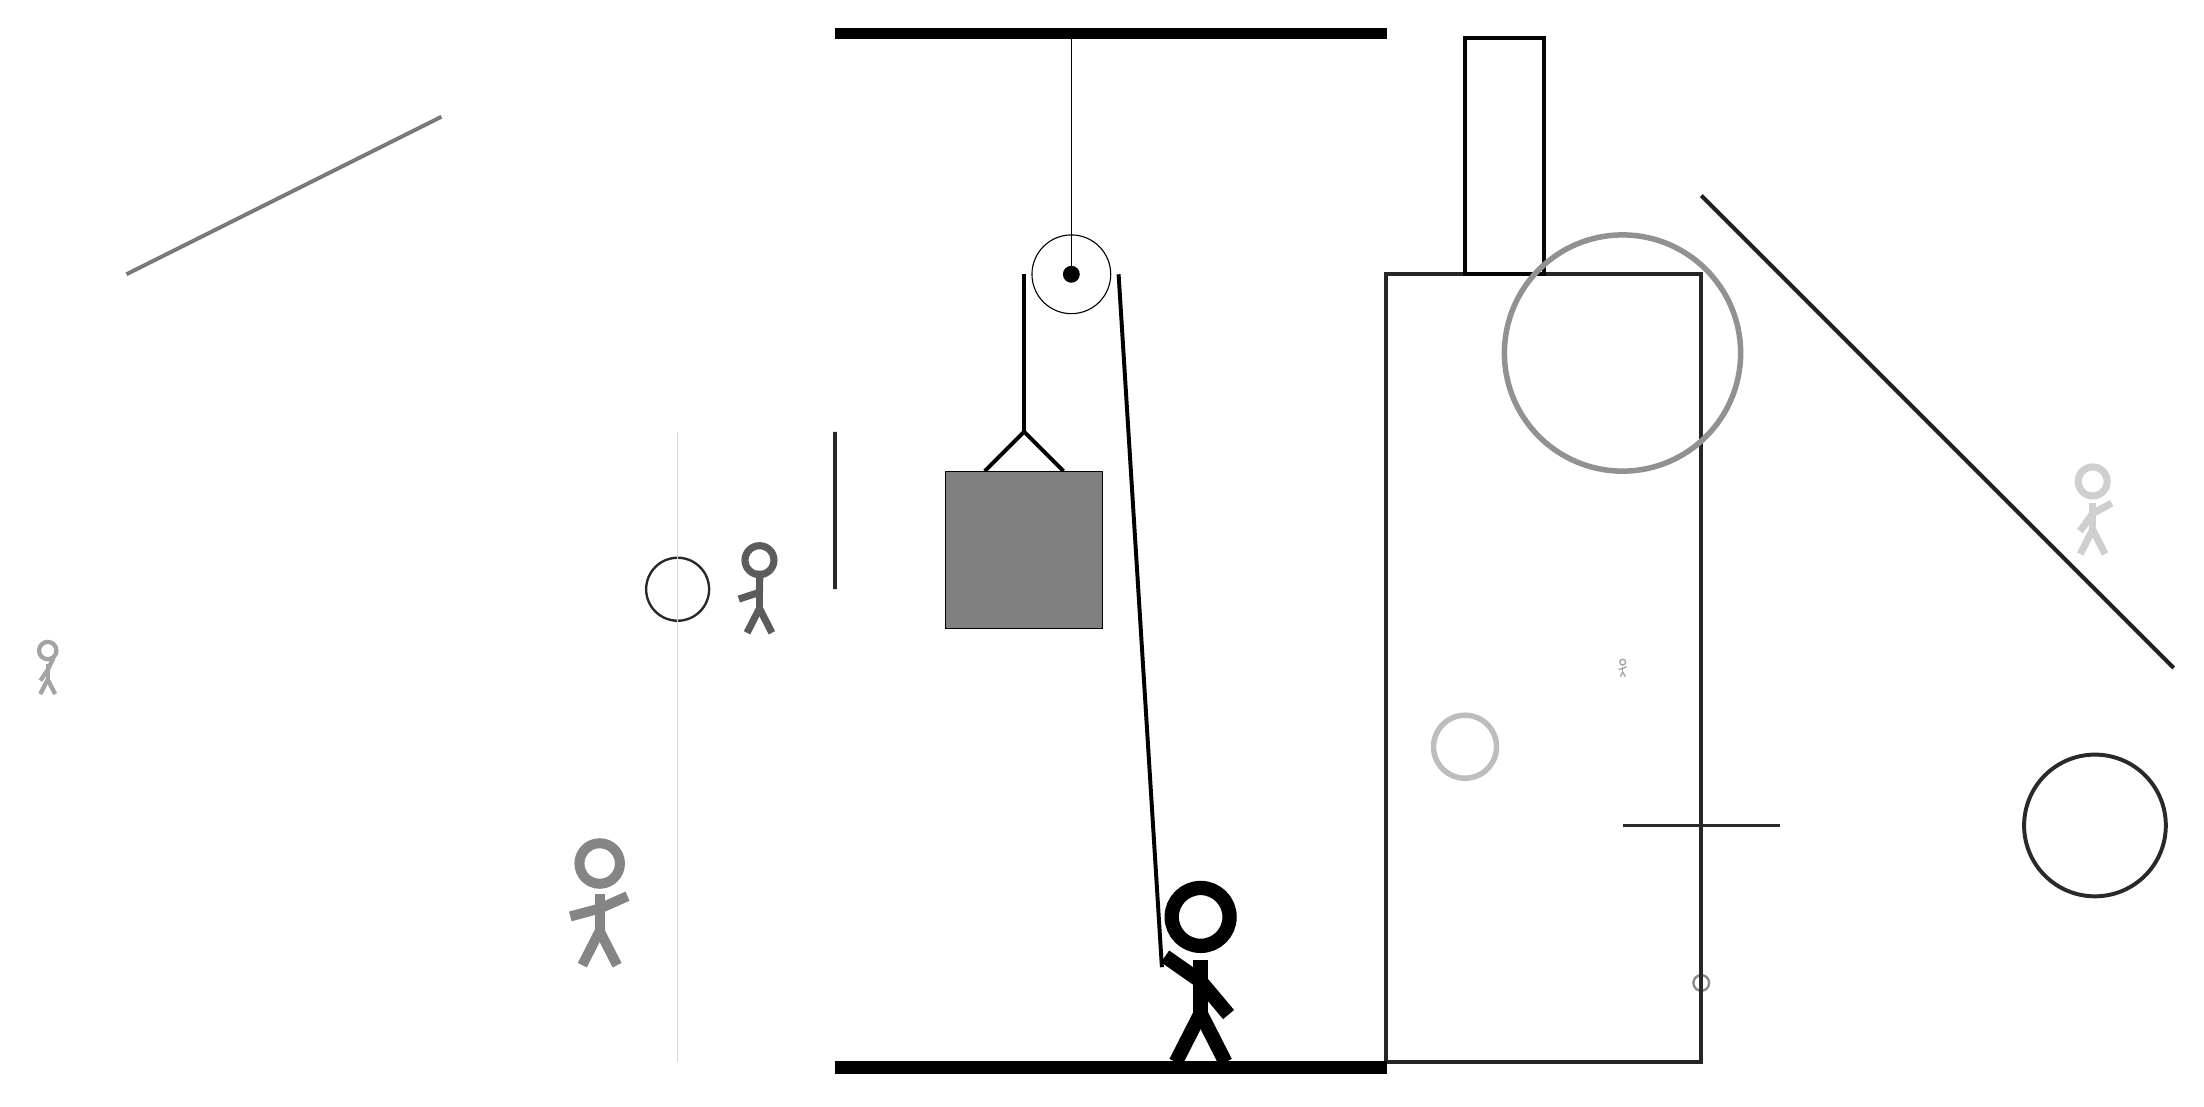
\begin{tikzpicture}
		%%%%% START %%%%%
		
		\draw[fill=black] (-2, 10) rectangle (5, 10.125);
		
		\draw (1, 7) circle (0.5);
		\draw[fill=black] (1, 7) circle (0.1);
		\draw (1, 10) -- (1, 7);
		
		\draw [line width=0.3mm, color=black!46](9, -2) circle (0.1);
		
		\node[line width=0.4mm, color=black!19] at (14, 4) {\Strichmaxerl[5][54][29]};
		\node[line width=0.6mm, color=black!36] at (-12, 2) {\Strichmaxerl[3][56][64]};
		\draw [line width=0.3mm, color=black!84](-4, 3) circle (0.4);
		\node[line width=0.7mm, color=black!48] at (-5, -1) {\Strichmaxerl[7][15][24]};
		\draw[line width=0.5mm, color=black!85] (5, 7) rectangle (9, -3);
		\draw [line width=0.7mm, color=black!26](6, 1) circle (0.4);
		\draw[line width=0.5mm, color=black!98] (7, 7) rectangle (6, 10);
		\draw [line width=0.7mm, color=black!43](8, 6) circle (1.5);
		\node[line width=0.2mm, color=black!64] at (-3, 3) {\Strichmaxerl[5][18][89]};
		
		\draw[line width=0.5mm, color=black!52](-7, 9) -- (-11, 7);
		\draw[line width=0.2mm, color=black!16] (-4, -3) rectangle (-4, 5);
		\draw [line width=0.6mm, color=black!66](8, -1) circle (0.0);
		\node[line width=0.6mm, color=black!34] at (8, 2) {\Strichmaxerl[1][12][28]};
		\draw[line width=0.5mm, color=black!83](10, 0) -- (8, 0);
		\draw [line width=0.5mm, color=black!84](14, 0) circle (0.9);
		
		\draw[line width=0.6mm, color=black!84] (-2, 5) rectangle (-2, 3);
		\draw[line width=0.5mm, color=black!88](9, 8) -- (15, 2);
		
		\draw[line width=0.5mm] (-0.1, 4.5) -- (0.4, 5.0) -- (0.9, 4.5);
		\draw[fill=black!50] (-0.6, 4.5) rectangle (1.4, 2.5);
		
		\draw[line width=0.5mm] (0.4, 7) -- (0.4, 5.0);
		\centerarc[line width=0.5mm](1, 7)(0:180:0.6);
		\draw[line width=0.5mm](1.6, 7) -- (2.15, -1.8);
		
		\node at (2.6, -1.9) {\Strichmaxerl[10][-35][-50]};
		
		\draw[fill=black] (-2, -3) rectangle (5, -3.15);
		
		%%%%% END %%%%%
	\end{tikzpicture}
\end{document}